\documentclass[12pt,fleqn]{article}
\usepackage{vkCourseML}
\hypersetup{unicode=true}
%\usepackage[a4paper]{geometry}
\usepackage[hyphenbreaks]{breakurl}

\interfootnotelinepenalty=10000

\begin{document}
\title{Лекция 13\\Ядровые методы}
\author{Е.\,А.\,Соколов\\ФКН ВШЭ}
\maketitle

\section{Ядровые методы}

Нам уже известно некоторое количество способов преобразования признаков:
можно добавлять признаки более высоких порядков, логарифмировать их или применять
другие нелинейные преобразования, отбирать с помощью~$L_1$-регуляризации
или, например, можно порождать новые признаки с помощью решающих деревьев.
На предыдущей лекции мы изучили метод главных компонент, который позволяет
формировать новые признаки как линейные комбинации исходных.
В данной лекции мы обсудим ещё один подход к изменению признакового пространства:
ядра, которые позволяют повышать размерность пространства без вычислительных трудностей.

\subsection{Восстановление нелинейных зависимостей линейными методами}
Линейные методы классификации и регрессии являются хорошо изученными
и обоснованными, однако предположение о линейной зависимости
зачастую оказывается неверным в задачах машинного обучения.
Оказывается, что линейные методы можно применять и для восстановления
нелинейных зависимостей, если предварительно перейти к новым признакам.

\begin{figure}[t]
\centering
\begin{multicols}{2}
    \hfill
    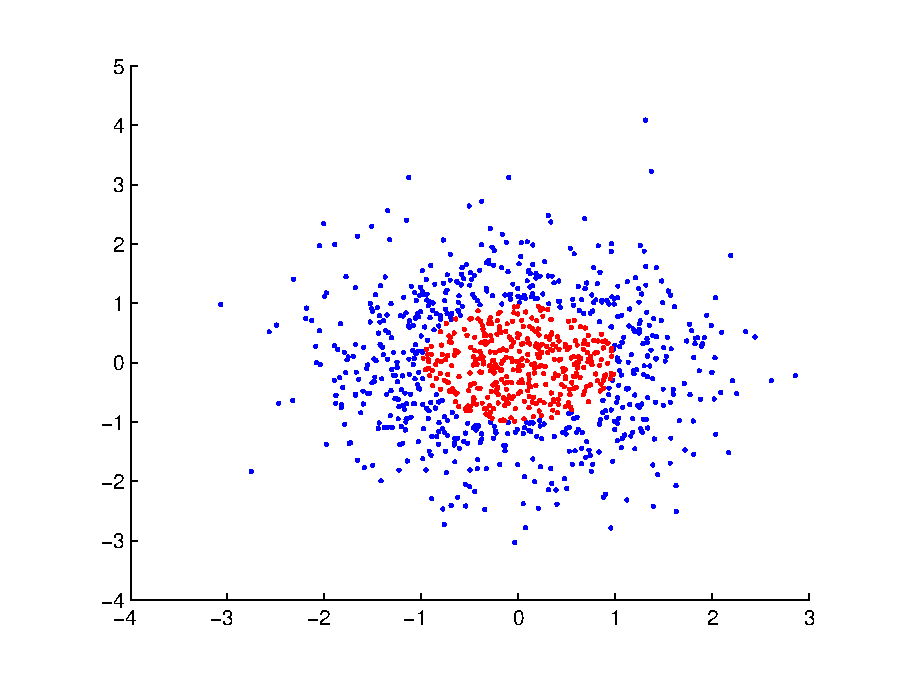
\includegraphics[width=0.9\linewidth]{example.eps}
    \hfill
    \caption{Выборка с нелинейной разделяющей поверхностью.
        Разные классы обозначены разными цветами.}
    \label{pic:nonlinSample}
    \hfill
    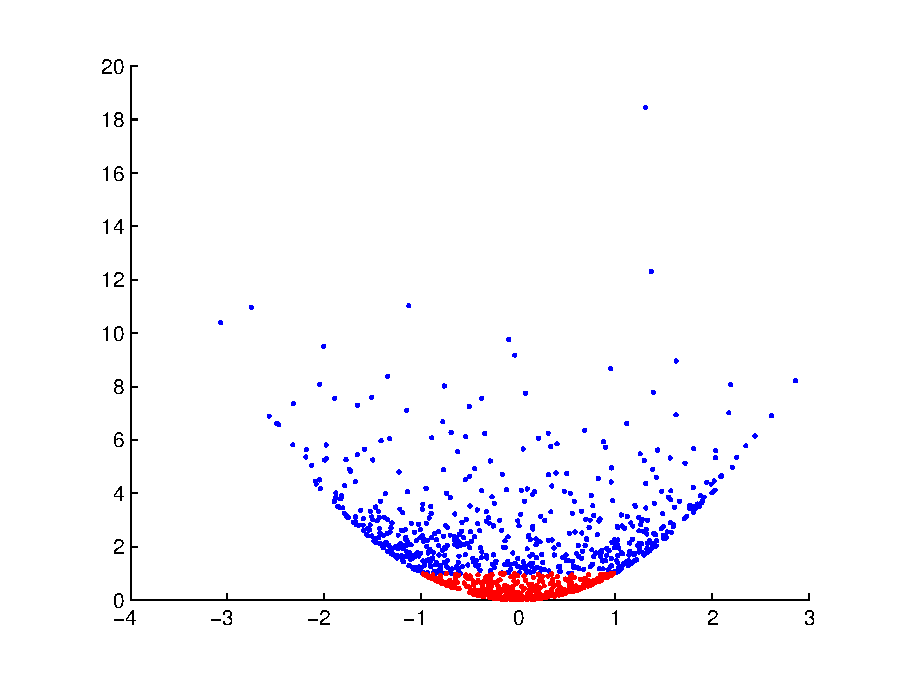
\includegraphics[width=0.9\linewidth]{example_newFeature.eps}
    \hfill
    \caption{Выборка после добавления третьего признака.
        Изображена проекция на первый и третий признаки.}
    \label{pic:nonlinSample_ext}
\end{multicols}
\end{figure}

Рассмотрим простой пример.
На рис.~\ref{pic:nonlinSample} показана двумерная выборка с двумя классами,
разделяющая поверхность для которой никак не может быть приближена гиперплоскостью.
В то же время, если добавить третий признак~$x_3 = x_1^2 + x_2^2$,
то выборку можно будет идеально разделить гиперплоскостью
вида~$x_3 = C$~(рис.~\ref{pic:nonlinSample_ext}).
Такое пространство называется~\emph{спрямляющим}.
В новом признаковом пространстве разделяющая поверхность является
линейной, однако после ее проецирования на исходное пространство
она окажется нелинейной.

Модель, в которой зависимость ищется как линейная комбинация
нелинейных функций от выборки, называется~\emph{линейной моделью над
базисными функциями}~\cite{bishop06prml}.
Например, для задачи регрессии она имеет вид
\[
    a(x) = \sum_{i = 1}^{m} w_i \phi_i(x),
\]
где~$\phi_i(x)$~--- произвольные нелинейные функции от
признаков~(\emph{базисные} функции).
Проблема заключается в том, что на практике
заранее нельзя сказать, какие именно базисные функции
нужно взять, чтобы добиться линейной разделимости, поэтому приходится
брать сразу большой набор таких функций~(например, все мономы не больше определенной
степени).
В этом случае число признаков оказывается очень большим,
из-за чего процесс обучения становится трудоемким как по времени, так и по памяти.
Однако в некоторых случаях оказывается, что достаточно уметь быстро
вычислять скалярные произведения объектов друг на друга.

\subsection{Двойственное представление для линейной регрессии}
Рассмотрим задачу построения линейной регрессии с квадратичной
функцией потерь и квадратичным регуляризатором:
\[
    Q(w)
    =
    \frac{1}{2} \sum_{i = 1}^{\ell} \Biggl\{
        \sum_{j = 1}^{m} w_j \phi_j(x_{i}) - y_i
    \Biggr\}^2
    +
    \frac{\lambda}{2} \|w\|^2
    =
    \frac{1}{2} \| \Phi w - y \|^2 + \frac{\lambda}{2} \|w\|^2 \to \min_w,
\]
где~$\Phi$~--- матрица, в которой~$i$-я строка представлена
вектором~$(\phi_1(x_i), \dots, \phi_m(x_i))$.
Дифференцируя функционал~$Q(w)$ и приравнивая его нулю,
получаем
\[
    w = - \frac{1}{\lambda}
        \Phi^T (\Phi w - y).
\]
Отсюда следует, что решение является линейной комбинацией
строк матрицы~$\Phi$:
\[
    w = \Phi^T a,
\]
где за~$a$ мы обозначили вектор~$-\frac{1}{\lambda} (\Phi w - y)$.
Подставим это представление в функционал:
\[
    Q(a)
    =
    \frac{1}{2} \| \Phi \Phi^T a - y \|^2 + \frac{\lambda}{2} a^T \Phi \Phi^T a \to \min_a.
\]
Заметим, что теперь функционал зависит не от самой матрицы признаков~$\Phi$,
а от ее произведения на саму себя~$\Phi \Phi^T$.
Это матрица скалярных произведений всех возможных пар объектов,
называемая также~\emph{матрицей Грама}.
Будем обозначать ее через
\[
    K = \Phi \Phi^T =
    (\langle \phi(x_i), \phi(x_j) \rangle)_{i, j = 1}^{\ell}
    =
    (k(x_i, x_j))_{i, j = 1}^{\ell},
\]
где~$\phi(x_i) = (\phi_1(x_i), \dots, \phi_m(x_i))$,
а~$k(x_i, x_j)$~--- скалярное произведение объектов,
называемое также~\emph{функцией ядра}.

Можно показать, что оптимальный вектор~$a$ имеет вид
\[
    a = (K + \lambda I)^{-1} y.
\]
Функция регрессии при этом запишется как
\[
    y(x)
    =
    \langle w, \phi(x) \rangle
    =
    w^T \phi(x)
    =
    a^T \Phi \phi(x)
    =
    k(x)^T (K + \lambda I)^{-1} y,
\]
где~$k(x) = (k(x, x_1), \dots, k(x, x_\ell))$~--- вектор скалярных произведений
нового объекта~$x$ на объекты обучающей выборки.

Итак, нам удалось переписать функционал и модель так, что они зависят лишь
от скалярных произведений объектов.
В этом случае при росте размерности нового~(спрямляющего) признакового пространства
количество требуемой памяти остается константным и имеет порядок~$\ell^2$.
Далее мы покажем, что и вычисление скалярного произведения
можно организовать так, что оно будет зависеть лишь от размерности
исходного признакового пространства.

\subsection{SVM и kernel trick}
Переход к новому признаковому пространству можно применять
и в задачах классификации:
\[
    a(x) = \sign ( \langle w, \phi(x) \rangle + b).
\]

В частности, к задаче метода опорных векторов можно построить двойственную:
\[
    \left\{
        \begin{aligned}
            & \sum_{i = 1}^{\ell}
                \lambda_i
            -
            \frac{1}{2} \sum_{i, j = 1}^{\ell}
                \lambda_i \lambda_j y_i y_j \langle x_i, x_j \rangle
            \to \max_{\lambda} \\
            & 0 \leq \lambda_i \leq C, \quad i = 1, \dots, \ell, \\
            & \sum_{i = 1}^{\ell} \lambda_i y_i = 0.
        \end{aligned}
    \right.
\]
После того, как она решена, новые объекты классифицируются
с помощью алгоритма
\[
    a(x) = \sign \left(
        \sum_{i = 1}^{\ell} \lambda_i y_i \langle x_i, x \rangle + b
    \right).
\]
Заметим, что как оптимизационная задача, так и итоговый классификатор
зависят лишь от скалярных произведений объектов.
Подставляя вместо скалярного произведения функцию ядра,
мы будем настраивать классификатор в произвольном признаковом пространстве.
Такая подмена получила в англоязычной литературе
название~\emph{kernel trick}.

\subsection{Ядра}
\emph{Ядром} мы будем называть функцию~$K(x, z)$,
представимую в виде скалярного произведения в некотором
пространстве:~$K(x, z) = \langle \phi(x), \phi(z) \rangle$,
где~$\phi: X \to H$~--- отображение из исходного признакового пространства
в некоторое~\emph{спрямляющее пространство}.
На семинарах будет показано, что ядро содержит в себе много информации о спрямляющем пространстве
и позволяет производить в нем различные операции, не зная самого
отображения~$\phi(x)$~--- например, находить расстояния между векторами~$\phi(x)$.

\subsubsection{Построение ядер}
Самый простой способ задать ядро~--- в явном виде построить
отображение~$\phi(x)$ в спрямляющее признаковое пространство.
Тогда ядро определяется как скалярное произведение в этом
пространстве: $K(x, z) = \langle \phi(x), \phi(z) \rangle$.
При таком способе, однако, возникают проблемы с ростом вычислительной сложности,
о которых уже было сказано выше.

Допустим, в качестве новых признаков мы хотим взять всевозможные
произведения исходных признаков.
Определим соответствующее отображение
\[
    \phi(x)
    =
    (x_i x_j)_{i, j = 1}^{d}
    \in
    \RR^{d^2}
\]
и найдем ядро:
\begin{align*}
    K(x, z)
    &=
    \langle \phi(x), \phi(z) \rangle
    =
    \langle (x_i x_j)_{i, j = 1}^{d}, (z_i z_j)_{i, j = 1}^{d} \rangle
    =\\
    &=
    \sum_{i, j = 1}^{d}
        x_i x_j z_i z_j
    =\\
    &=
    \sum_{i = 1}^{d} x_i z_i
    \sum_{j = 1}^{d} x_j z_j
    =\\
    &=
    \langle x, z \rangle^2.
\end{align*}
Таким образом, ядро выражается через скалярное произведение
в исходном пространстве,
и для его вычисления необходимо порядка~$d$ операций~(в то время
как прямое вычисление ядра потребовало бы~$O(d^2)$ операций).

\subsubsection{Неявное задание ядра}
Пример с мономами показал, что можно определить ядро так,
что оно не будет в явном виде использовать отображение объектов
в новое признаковое пространство.
Но как убедиться, что функция~$K(x, z)$ определяет скалярное
произведение в некотором пространстве?
Ответ на этот вопрос дает~\emph{теорема Мерсера}:
функция~$K(x, z)$ является ядром тогда и только тогда, когда:
\begin{enumerate}
    \item Она симметрична: $K(x, z) = K(z, x)$.
    \item Она неотрицательно определена, то есть для
        любой конечной выборки~$(x_1, \dots, x_\ell)$
        матрица~$K = \bigl( K(x_i, x_j) \bigr)_{i, j = 1}^{\ell}$
        неотрицательно определена.
\end{enumerate}

Проверять условия теоремы Мерсера, однако, может быть достаточно трудно.
Поэтому для построения ядер, как правило, пользуются несколькими базовыми
ядрами и операциями над ними, сохраняющими симметричность и неотрицательную
определенность.
\begin{vkTheorem}[\cite{shawetaylor04kernels}]
\label{th:kernelConstr}
    Пусть~$K_1(x, z)$ и~$K_2(x, z)$~--- ядра, заданные на множестве~$X$,
    $f(x)$~--- вещественная функция на~$X$,
    $\phi: X \to \RR^N$~--- векторная функция на~$X$,
    $K_3$~--- ядро, заданное на~$\RR^N$.
    Тогда следующие функции являются ядрами:
    \begin{enumerate}
        \item $K(x, z) = K_1(x, z) + K_2(x, z)$,
        \item $K(x, z) = \alpha K_1(x, z)$, $\alpha > 0$,
        \item $K(x, z) = K_1(x, z) K_2(x, z)$,
        \item $K(x, z) = f(x) f(z)$,
        \item $K(x, z) = K_3(\phi(x), \phi(z))$.
    \end{enumerate}
\end{vkTheorem}

\begin{vkTheorem}[\cite{sholkopf02kernels}]
\label{th:kernelLim}
    Пусть~$K_1(x, z), K_2(x, z), \dots$~--- последовательность ядер,
    причем предел
    \[
        K(x, z)
        =
        \lim_{n \to \infty}
            K_n(x, z)
    \]
    существует для всех~$x$ и~$z$.
    Тогда~$K(x, z)$~--- ядро.
\end{vkTheorem}

Рассмотрим некоторые примеры построения ядер.

\subsubsection{Полиномиальные ядра}
Пусть~$p(v)$~--- многочлен с положительными коэффициентами.
На семинарах будет показано, что~$K(x, z) = p(\langle x, z \rangle)$~--- ядро.
Также известно, что~$p(K(x, z))$~--- ядро для любого ядра~$K(x, z)$.

Рассмотрим частный случай полиномиального ядра:
\[
    K_m(x, z)
    =
    \left(
        \langle x, z \rangle + R
    \right)^m.
\]
Распишем степень, воспользовавшись формулой бинома Ньютона:
\[
    K_m(x, z)
    =
    \sum_{i = 0}^{m}
        C_m^i R^{m - i}
        \langle x, z \rangle^i.
\]
Поскольку коэффициенты при скалярных произведениях~$C_m^i R^{m - i}$
положительны, то данное ядро действительно является ядром.
Если расписать скалярные произведения, то можно убедиться,
что оно соответствует переводу набора признаков
во всевозможные мономы над признаками степени не больше~$m$,
причем моном степени~$i$ имеет вес~$\sqrt{C_m^i R^{m - i}}$.

Заметим, что параметр~$R$ контролирует относительный вес при мономах больших степеней.
Например, отношение веса при мономе степени~$m - 1$ к весу при мономе первой степени
равно
\[
    \sqrt{\frac{C_{m}^{m - 1} R}{C_{m}^{1} R^{m - 1}}}
    =
    \sqrt{\frac{1}{R^{m - 2}}},
\]
то есть по мере увеличения~$R$ вес при мономах старших степеней
будет становиться очень небольшим по сравнению с весом при остальных мономах.
Можно сказать, что параметр~$R$ контролирует сложность модели.

\subsubsection{Гауссовские ядра}
Гауссовское ядро определяется как
\[
    K(x, z) = \exp\left( -\frac{\|x - z\|^2}{2 \sigma^2} \right).
\]
Покажем, что оно действительно является ядром.

Покажем сначала, что функция~$\exp(\langle x, z \rangle)$
является ядром.
Представим ее в виде предела последовательности:
\[
    \exp(\langle x, z \rangle)
    =
    \sum_{k = 0}^{\infty}
        \frac{\langle x, z \rangle^k}{k!}
    =
    \lim_{n \to \infty}
        \sum_{k = 0}^{n}
            \frac{\langle x, z \rangle^k}{k!}.
\]
Каждый член предельной последовательности является многочленом
с положительными коэффициентами, и поэтому является ядром.
Предел существует во всех точках~$(x, z)$, поскольку
ряд Тейлора для функции~$e^x$ сходится на всей числовой прямой.
Значит, по теореме~\ref{th:kernelLim} данная функция является ядром.

Аналогично можно доказать, что функция~$\exp(\langle x, z \rangle / \sigma^2)$
также является ядром.
Гауссовское ядро легко получить из данного путём замены преобразования~$\phi(x)$
на~$\phi(x) / \|\phi(x)\|$.

Заметим, что можно построить гауссово ядро, используя любое
другое ядро~$K(x, z)$.
В этом случае оно примет вид
\[
    \exp\left( -\frac{\|\phi(x) - \phi(z)\|^2}{2 \sigma^2} \right)
    =
    \exp\left(
    -\frac{
        K(x, x) - 2 K(x, z) + K(z, z)
    }{
        2 \sigma^2
    }
    \right).
\]
Здесь мы расписали расстояние между векторами~$\|\phi(x) - \phi(z)\|^2$
в спрямляющем пространстве через функцию ядра.

\paragraph{Спрямляющее пространство.}
Какому спрямляющему пространству соответствует гауссовское ядро?
Оно является пределом последовательности полиномиальных ядер
при стремлении степени ядра к бесконечности,
что наталкивает на мысль, что и спрямляющее пространство
будет бесконечномерным.
Чтобы показать это формально, нам понадобится следующее утверждение.

\begin{vkState}[\cite{micchelli86interpolation}]
\label{th:gaussGram}
    Пусть~$x_1, \dots, x_\ell$~--- различные точки пространства~$\RR^d$.
    Тогда матрица
    \[
        G = \left[
            \exp\left(
                -\frac{
                    \|x_i - x_j\|^2
                }{
                    2 \sigma^2
                }
            \right)
        \right]_{i, j = 1}^{\ell}
    \]
    является невырожденной при~$\sigma > 0$.
\end{vkState}

Вспомним также факт из линейной алгебры: матрица Грама системы точек~$x_1, \dots, x_\ell$
невырождена тогда и только тогда, когда эти точки линейно независимы.
Поскольку матрица из утверждения~\ref{th:gaussGram} является матрицей Грама
для точек~$x_1, \dots, x_\ell$ в спрямляющем пространстве гауссова ядра,
то заключаем, что в данном пространстве существует сколь угодно много
линейно независимых точек.
Значит, данное пространство является бесконечномерным.

Можно показать это и менее формально.
Распишем функцию ядра:
\begin{align*}
    K(x, z)
    &=
    \exp\left(
        -\frac{
            \|x - z\|^2
        }{
            2 \sigma^2
        }
    \right)
    =
    \exp\left(
        -\frac{
            \|x\|^2
        }{
            2 \sigma^2
        }
    \right)
    \exp\left(
        -\frac{
            \|z\|^2
        }{
            2 \sigma^2
        }
    \right)
    \exp\left(
        -\frac{
            \langle x, z \rangle
        }{
            \sigma^2
        }
    \right)
    =\\
    &=
    \{\text{раскладываем экспоненту в ряд}\}
    =\\
    &=
    \exp\left(
        -\frac{
            \|x\|^2
        }{
            2 \sigma^2
        }
    \right)
    \exp\left(
        -\frac{
            \|z\|^2
        }{
            2 \sigma^2
        }
    \right)
    \sum_{k = 0}^{\infty}
        \frac{
            \langle x, z \rangle^k
        }{
            k! \sigma^{2k}
        }.
\end{align*}
Легко видеть, что для получения~$k$-го слагаемого в спрямляющем пространстве
должны быть все мономы степени~$k$ над исходными признаками.
Поскольку всего в сумме бесконечное число слагаемых, то и размерность
спрямляющего пространства должна быть бесконечной.

\paragraph{Роль параметра~$\sigma$.}
Заметим, что параметр~$\sigma$ в разложении гауссова ядра
в ряд Тейлора входит в коэффициент перед слагаемым~$\langle x, z \rangle^k$
как~$1 / \sigma^{2k}$.
Его роль аналогична параметру~$R$ в полиномиальных ядрах.
Маленькие значения~$\sigma$ соответствуют большим значениям~$R$:
чем меньше~$\sigma$, тем больше вес при мономах большой степени, тем
больше риск переобучения.


\begin{thebibliography}{1}
\bibitem{bishop06prml}
    \emph{Bishop, C.M.}
    Pattern Recognition and Machine Learning.~//
    Springer, 2006.

\bibitem{shawetaylor04kernels}
    \emph{Shawe-Taylor, J., Cristianini, N.}
    Kernel Methods for Pattern Analysis.~//
    Cambridge University Press, 2004.

\bibitem{sholkopf02kernels}
    \emph{Sholkopf, B.A., Smola, A.J.}
    Learning with kernels.~//
    MIT Press, 2002.

\bibitem{micchelli86interpolation}
    \emph{Micchelli, C.A.}
    Algebraic aspects of interpolation.~//
    Proceedings of Symposia in Applied Mathematics, 36:81-102, 1986.
\end{thebibliography}



\end{document}
